\documentclass[tikz,border=10pt]{standalone}
\usepackage{amsmath}
\begin{document}
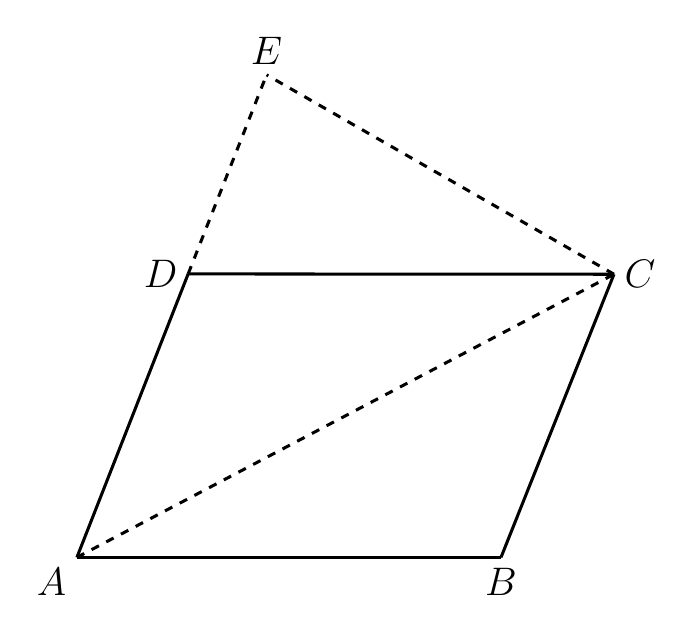
\begin{tikzpicture}[line join=round, line width=1.1pt]
\coordinate (A) at (-3.431,-3.229);
\coordinate (B) at (1.955,-3.229);
\coordinate (C) at (3.390,0.367);
\coordinate (D) at (-2.018,0.371);



\coordinate (E) at (-1.022,2.899);


\draw (A) -- (B);
\draw (B) -- (C);
\draw (C) -- (D);
\draw (A) -- (D);


\draw[dashed] (D) -- (E);
\draw[dashed] (C) -- (E);
\draw[dashed] (A) -- (C);


\node[below left, font=\fontsize{15}{18}\selectfont] at (A) {$A$};
\node[below, font=\fontsize{15}{18}\selectfont] at (B) {$B$};
\node[right, font=\fontsize{15}{18}\selectfont] at (C) {$C$};
\node[left, font=\fontsize{15}{18}\selectfont] at (D) {$D$};
\node[above, font=\fontsize{15}{18}\selectfont] at (E) {$E$};
\end{tikzpicture}
\end{document}